
%\section{Contended Data Structures}
\section{Contended Data Structures}
\label{section:contended}
In this section, we consider data structures that are often contended when accessed 
by many threads concurrently. In these data structures, operations compete for accessing one or more 
locations, creating a contention spot, which can become a performance bottleneck.
Examples include head and tail pointers in queues or the top pointer of a stack.

These data structures have good locality; therefore, the contention spots are often found 
in shared CPU caches, such as the last-level cache in a multi-socket machine 
when shared by threads running on a single socket. Therefore, these data structures might 
seem to be a poor fit for near-memory computing: the advantage of faster memory access provided by PIM 
cannot be exercised because the frequently accessed data might stay in the CPU cache. 
However, such a perspective does not consider the overhead introduced by contention 
in a concurrent data structure where \emph{many} threads access the \emph{same} locations. 

As a representative example of this class of data structures, we consider a FIFO queue, 
where concurrent enqueue
and dequeue operations compete for the head and the tail of the queue, respectively. 
Although a naive PIM FIFO queue is not a good replacement for a well crafted concurrent FIFO queue, 
we show that, counterintuitively, PIM can still have benefits over a traditional concurrent FIFO 
queue. In particular, we exploit the \emph{pipelining} of requests from CPUs, 
which can be done very efficiently in PIM, to design a PIM FIFO queue that can outperform 
state-of-the-art concurrent FIFO queues, such as the flat-combining FIFO queue~\cite{Hendler10} 
and the F\&A FIFO queue~\cite{Morrison13}.

\subsection{FIFO queues}
The structure of our PIM-managed FIFO queue is shown in Figure \ref{figure:queue_structure}.
A queue consists of a sequence of \emph{segments}, each containing consecutive nodes of the queue.
A segment is allocated in a PIM vault, with a head node and a tail node pointing to the first 
and the last nodes of the segment, respectively.
A vault can contain multiple (likely non-consecutive) segments. 
There are two special segments---the \textit{enqueue segment} and the \textit{dequeue segment}.
To enqueue a node, a CPU sends an enqueue request to the PIM core of the vault 
containing the enqueue segment.
The PIM core then inserts the node to the head of the segment.
Similarly, to dequeue a node, a CPU sends a dequeue request to the PIM core of the vault
holding the dequeue segment. 
The PIM core then removes the node at the tail of the dequeue segment and 
sends the node back to the CPU.

\begin{figure}[ht!]
%$\hrulefill$
%\\
%\\
\centering
\includegraphics[width=.95\linewidth]{queue_structure.eps}
%$\hrulefill$
\caption{A PIM-managed FIFO queue with three segments}
\label{figure:queue_structure}
\end{figure}

\begin{algorithm*}[ht!]
{\footnotesize
%scriptsize
\caption{PIM-managed FIFO queue}
\label{alg:queue}
\vspace{-2.5ex}
\begin{multicols}{2}
\begin{algorithmic}[1]
\Procedure{enq}{cid, $u$}
	\If{enqSeg == null}
        \State send message(cid, false);
    \Else
        \If{enqSeg.head $\ne$ null}
            \State enqSeg.head.next = $u$;
            \State enqSeg.head = $u$;
        \Else
            \State enqSeg.head = $u$;
            \State enqSeg.tail = $u$;
        \EndIf

        \State enqSeg.count = enqSeg.count + 1;
        \State send message(cid, true);

        \If{enqSeg.count $>$ threshold}
            \State cid$'$ = the CID of the PIM core chosen to maintain the new segment;
            \State send message(cid$'$, newEnqSeg());
            \State enqSeg.nextSegCid = cid$'$;
            \State enqSeg = null;
        \EndIf
    \EndIf
\item[]
\EndProcedure
\algstore{}
\end{algorithmic}

\begin{algorithmic}[1]
\algrestore{}
\Procedure{newEnqSeg}{\null}
	\State enqSeg = new Segment();
	\State segQueue.enq(engSeg) ;
	\State notify the CPUs of the new enqueue segment;
\EndProcedure
\algstore{}
\end{algorithmic}
\columnbreak

\begin{algorithmic}[1]
\algrestore{}
\Procedure{deq}{cid}
	\If{deqSeg == null}
        \State send message(cid, false);
    \Else
        \If {deqSeg.tail $\ne$ null}
			\State send message(cid, deqSeg.tail);
            \State deqSeg.tail = deqSeg.tail.next;   
        \Else
			\If {deqSeg == enqSeg}
				\State send message(cid, null);
			\Else
                \State send message(deqSeg.nextSegCid, newDeqSeg());
                \State deqSeg = null;
                \State send message(cid, false);
            \EndIf            
        \EndIf 
    \EndIf     
\item[]
%\item[]
%\item[]
%\item[]
%\item[]
\EndProcedure
\algstore{}
\end{algorithmic}

\begin{algorithmic}[1]
\algrestore{}
\Procedure{newDeqSeg}{\null}
	\State deqSeg = segQueue.deq();
	\State notify the CPUs of the new dequeue segment; 
\EndProcedure
\end{algorithmic}

\end{multicols}
}
\vspace{-2ex}
\end{algorithm*}

Initially, the queue consists of an empty segment that acts as both the enqueue segment and 
the dequeue segment. 
When the length of the enqueue segment exceeds some threshold, the PIM core maintaining it
notifies another PIM core to create a new segment as the new enqueue segment.\footnote{
Alternative designs where a CPU decides when to create new segments based on more complex 
criteria are also possible. 
We leave such designs as future work. }
When the dequeue segment becomes empty and the queue has other segments, 
the dequeue segment is deleted and the segment that was created first 
among all the remaining segments is designated as the new dequeue segment. 
This segment was created when the old dequeue segment 
acted as the enqueue segment and exceeded the length threshold.
If the enqueue segment is different from the dequeue segment, 
enqueue and dequeue operations can be executed by two different PIM cores 
in parallel, improving the throughput. 
The F\&A queue~\cite{Morrison13} also allows parallel enqueue and dequeue. 

The pseudocode of the algorithm is presented in Algorithm \ref{alg:queue}. 
Each PIM core has local variables \textit{enqSeg} and \textit{deqSeg} that are references to 
local enqueue and dequeue segments.
When \textit{enqSeg} (or \textit{deqSeg}) is not null, it indicates that the PIM core is currently 
holding the enqueue (or dequeue) segment.
Each PIM core also maintains a local queue \textit{segQueue} for storing local segments.
CPUs and PIM cores communicate via message(\textit{cid}, \textit{content}) calls, 
where \textit{cid} is the unique core ID (CID) 
of the receiver and \textit{content} is either a request or a response to a request.

Once a PIM core receives an \emph{enqueue} request enq(\textit{cid}, $u$) of node $u$ from a CPU whose CID is \textit{cid},
it first checks if it is holding the enqueue segment (line 2 of Procedure enq(\textit{cid}, $u$)).
If so, the PIM core enqueues $u$ (lines 5-12), and otherwise sends back a message
informing the CPU that the request is rejected (line 3) so that
the CPU can resend its request to the right PIM core holding the enqueue segment
(we will explain later how the CPU can find the right PIM core).
After enqueuing $u$, the PIM core may find that the enqueue segment is longer than the threshold (line 13).
If so, it sends a message with a newEnqSeg() request to the PIM core of another vault that is chosen 
to create a new enqueue segment.
The PIM core then sets its \textit{enqSeg} to null, indicating that it no longer deals with enqueue operations.
Note that the CID \textit{cid} of the PIM core chosen for creating the new segment is recorded in 
\textit{enqSeg.nextSegCid} for future use in dequeue requests.
As Procedure newEnqSeg() in Algorithm \ref{alg:queue} shows,
The PIM core receiving this newEnqSeg() request creates a new enqueue segment and 
enqueues the segment into its \textit{segQueue} (line 3).
Finally, it notifies the CPUs of the new enqueue segment 
(we will discuss this notification in more detail later in this section).

Similarly, when a PIM core receives a \emph{dequeue} request deq(\textit{cid}) from a CPU with CID \textit{cid},
it first checks whether it is holding the dequeue segment (line 2 of Procedure deq(\textit{cid})).
If so, the PIM core dequeues a node and sends it back to the CPU (lines 5-7).
Otherwise, it informs the CPU that this request has failed (line 3) and
the CPU will have to resend its request to the right PIM core.
If the dequeue segment is empty (line 8) and the dequeue segment is not the same as 
the enqueue segment (line 11), so the FIFO queue is not empty, 
the PIM core sends a message with a newDeqSeg() request 
to the PIM core with CID \textit{deqSeg.nextSegCid}. 
We know that this PIM core must hold the next segment, 
according to how we create new segments in enqueue operations, 
as shown in lines 14-16 of Procedure enq(\textit{cid}, $u$). 
Upon receiving the newDeqSeg() request, 
the PIM core retrieves from its \textit{segQueue} the oldest segment it has created and 
makes it the new dequeue segment (line 2). 
Finally the PIM core notifies the CPUs that it is holding the new dequeue segment now.

We now explain how CPUs and PIM cores coordinate to make sure that the CPUs can find the right enqueue 
and dequeue segments, when their attempts fail due to enqueue/dequeue segment changes. 
We only discuss how to deal with enqueue segments, 
because the same methods can be applied to dequeue segments. 
A straightforward way to inform the CPUs is to have the owner PIM core of the new enqueue segment 
send notification messages to them (line 4 of newEngSeg()) 
and wait until all the CPUs send back acknowledgment messages. 
However, if there is a slow CPU core that doesn't reply in time, 
the PIM core has to wait for it and therefore other CPUs cannot have their requests executed. 
A more efficient, non-blocking method is to have the PIM core start serving new requests 
immediately after it has sent off the notifications to all CPUs. 
A CPU does not have to reply to those notifications in this case, 
but if its request later fails, it needs to send messages to all PIM cores 
to ask which PIM core is currently in charge of the enqueue segment.
In either case, the correctness of the algorithm is guaranteed:  
at any time, there is only one enqueue segment and only one dequeue segment; 
only requests sent to them will be executed. 
  
The PIM-managed FIFO queue can be further optimized. 
For example, the PIM core holding the enqueue segment can combine multiple pending enqueue requests 
and store the nodes to be enqueued in an array as a ``fat" node of the queue, 
in order to reduce memory accesses. 
This optimization is also used in the flat-combining FIFO queue \cite{Hendler10}. 
Even without this optimization, our algorithm still performs well, as we will show next. 

\subsection{Pipelining and Performance Analysis}
We compare the performance of three concurrent FIFO queues---our PIM-managed FIFO queue, 
the flat-combining FIFO queue and the F\&A-based FIFO queue \cite{Morrison13}. 
The F\&A-based FIFO queue is the most efficient concurrent FIFO queue we are aware of, 
where threads perform F\&A operations on two shared variables, 
one for enqueues and the other for dequeues, to compete for slots in the FIFO queue to 
enqueue and dequeue nodes (see \cite{Morrison13} for more details). 
The flat-combining FIFO queue we consider is based on the one proposed by \cite{Hendler10}, 
with a modification that threads compete for two ``combiner locks", 
one for enqueues and the other for dequeues. 
We further simplify it based on the assumption that the queue is always non-empty, 
so that it doesn't have to deal with synchronization issues between enqueues and dequeues 
when the queue is empty. These assumptions give an advantage to the flat combining queue, 
to make it competitive with the two other queues, which can perform parallel enqueue and dequeue. 

Let us first assume that a queue is long enough such that the PIM-managed FIFO queue 
has more than one segment, and enqueue and dequeue requests can be executed separately. 
Since enqueue/dequeue segment changes are infrequent, 
the overhead of such changes is negligible and therefore not included in our analysis.
For example, if the threshold of segment length in line 13 of enq(\textit{cid}, $u$) is a large integer $n$, 
then, in the worst case, changing an enqueue or dequeue segment happens only once every $n$ requests.
Moreover, a segment change only entails sending one message and a few steps of local computation.
In our analysis, we focus on dequeue operations, because 
 enqueues and dequeues are isolated from each other in all three algorithms when queues are long enough.
 The analysis of enqueues is similar. 

Assume there are $p$ concurrent dequeue requests by $p$ threads. 
In the F\&A algorithm, each thread needs to perform a F\&A operation on a shared variable, 
serializing access to this shared variable. 
Therefore, 
the execution time of $p$ requests is at least $p\latato$. 
If we assume that each CPU makes a request immediately after its previous request completes, 
the throughput (per second) of the algorithm is at most ${1 \over \latato}$. 

The flat-combining FIFO queue maintains a sequential FIFO queue and 
threads submit their requests into a \emph{publication list}. 
The publication list consists of slots, one for each thread, to store their requests.
After writing a request into the list, a thread competes with others for acquiring a lock 
to become the ``\emph{combiner}", which incurs one last-level cache access. 
The combiner then goes through the publication list to retrieve requests, executes operations for those requests, 
and writes results back to the list, while other threads with pending requests spin on their own slots, 
waiting for the results. 
The combiner therefore makes two last-level cache accesses\footnote{We assume the combiner finds the slots 
in the last-level cache, to the benefit of the flat combining algorithm. If the slots are not found in cache, 
the cost will be higher, as the combiner will incur memory accesses instead.} to each slot other than its own, 
one for reading the request and one for writing the result back. 
Thus, the execution time of $p$ requests in the algorithm is at least $(2p-1)\latllc$ and 
the throughput (per second) of the algorithm is at most ${1 \over 2\latllc}$ for large enough $p$.

Note that our analysis of the F\&A-based and the flat-combining algorithms is performed in favor of these 
algorithms, 
as we consider only partial costs of their executions. 
We have ignored the latency of accessing and modifying queue nodes in the two algorithms. 
For dequeues, this latency can be high: nodes to be dequeued in a long queue are unlikely 
to be cached, so the combiner has to perform a sequence of memory accesses to dequeue them one by one.  
Moreover, the F\&A-based algorithm may also suffer performance degradation under heavy contention, 
because contended F\&A operations may perform worse in practice \cite{David13}.

The performance of our PIM-managed FIFO queue seems poor at first sight: although a PIM core can update 
the queue efficiently, it takes a lot of time for the PIM core to send results back to CPUs one by one. 
To improve its performance, the PIM core can \textit{pipeline} the execution of requests, 
as illustrated in Figure \ref{figure:queue_pipeline}(a). 
Suppose $p$ CPUs send $p$ dequeue requests concurrently to the PIM core. 
The PIM core then retrieves a request from its message buffer (step 1 in the figure), 
dequeues a node (step 2) for the request, and sends the node back to the CPU (step 3). 
We can hide the message latency in step 3 as follows. 
After sending the message containing the node in step 3, the PIM core \emph{immediately} retrieves the next 
request to execute, without blocking to wait for the previous message to arrive at its receiver. 
This way, the PIM core \emph{pipelines} requests by overlapping the latency of message transfer in step 3  
and the latency of memory accesses and local computations in steps 1 and 2 across multiple requests 
(see Figure \ref{figure:queue_pipeline}(b)). 
Note that the PIM core still executes everything sequentially: 
it first sends the message for the current request before serving the next one.

\begin{figure}[ht!]
%$\hrulefill$
%\\
%\\
\centering
\subfigure[]{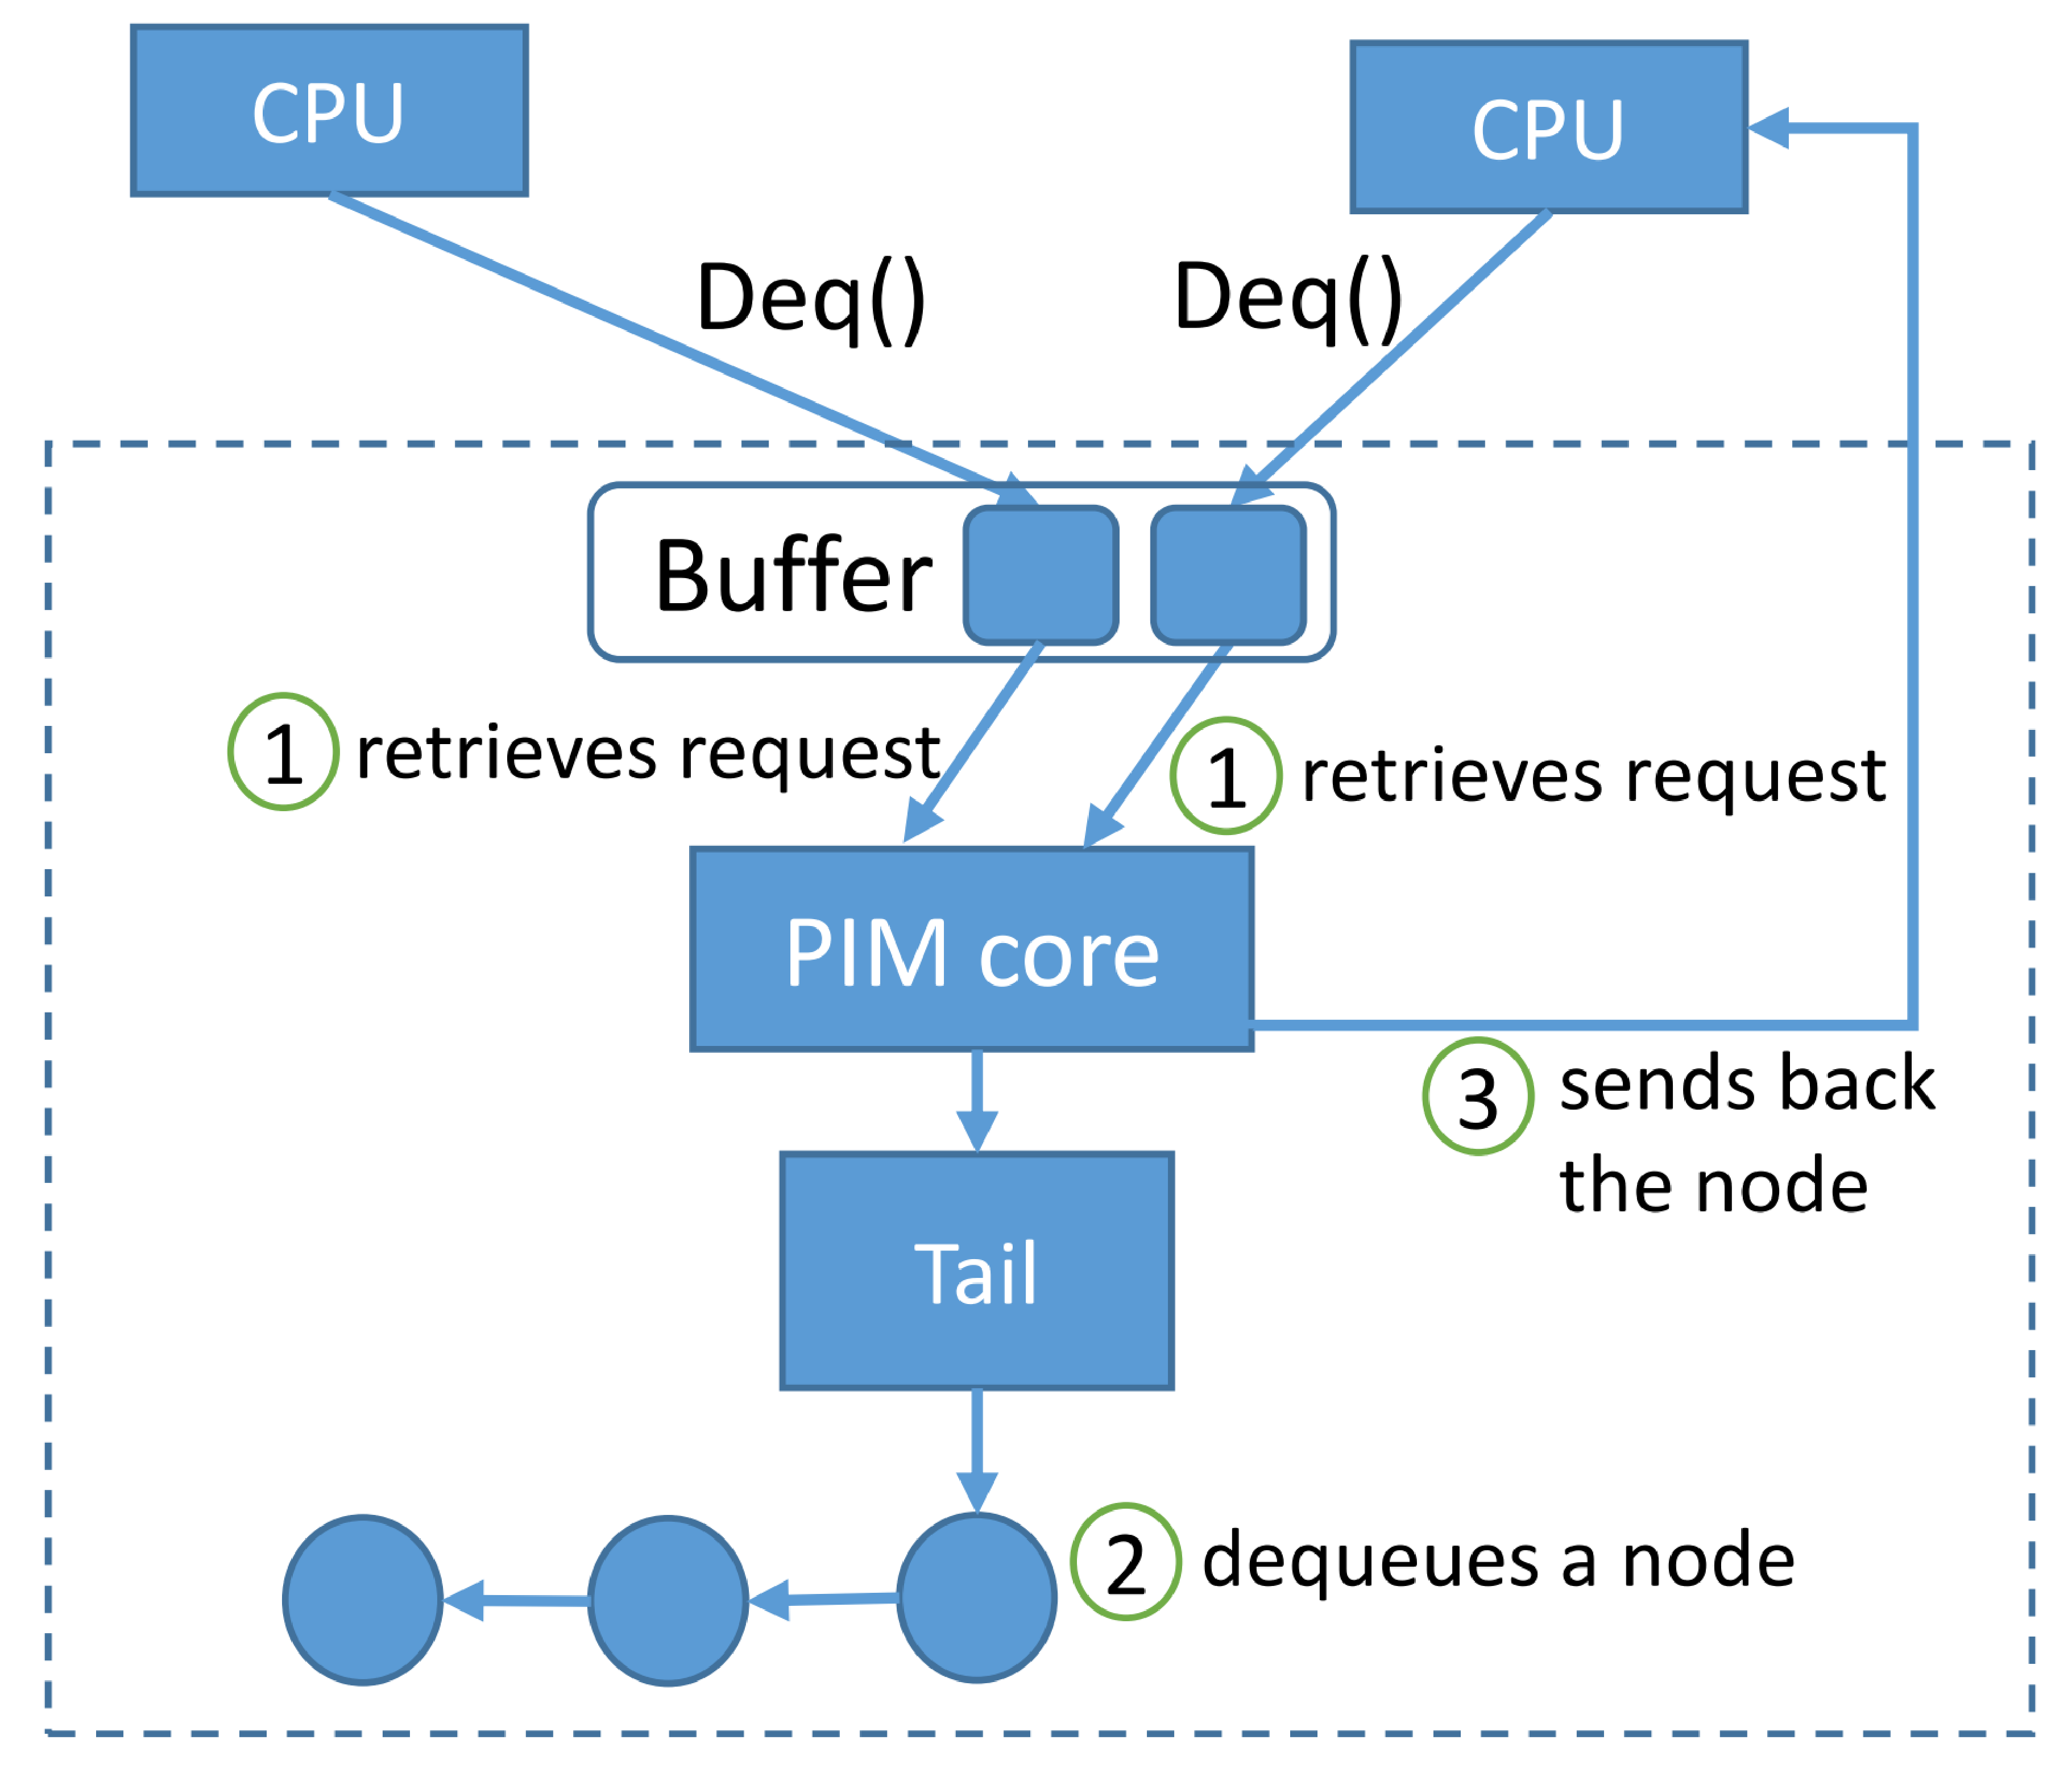
\includegraphics[width=.6\linewidth]{queue_pipeline.eps}}
\\
\subfigure[]{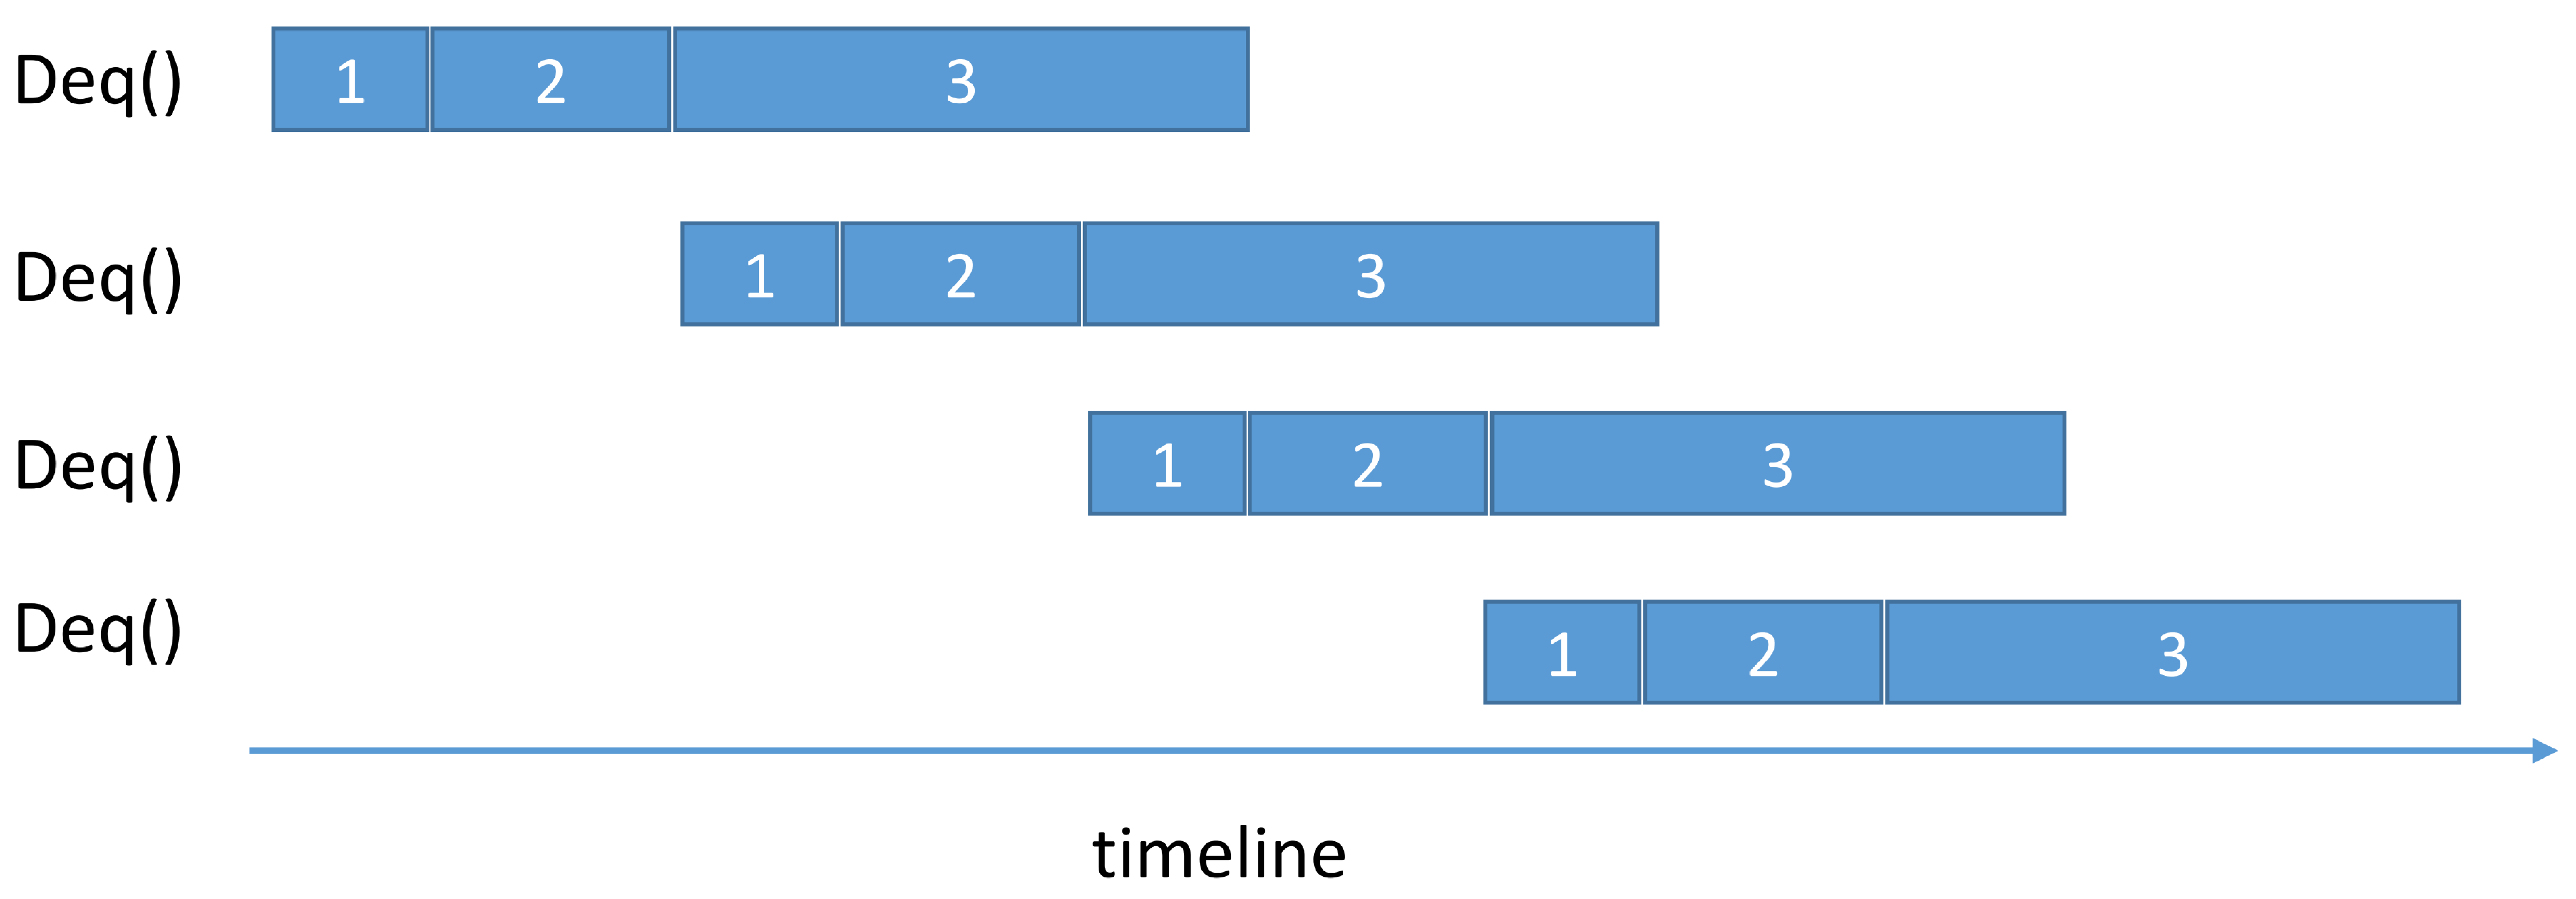
\includegraphics[width=.7\linewidth]{queue_pipeline_timeline.eps}}

%$\hrulefill$
\caption{(a) The pipelining optimization, where a PIM core can start executing 
a new deq() (step 1 of deq() for CPU B), without waiting for the dequeued node of 
the previous deq() to return to CPU A (step 3). 
(b) The timeline of pipelining four deq() requests.}
\label{figure:queue_pipeline}
\end{figure}
 
The throughput of a PIM core is given by the costs of its memory accesses and local computations, 
as long as it has enough bandwidth to keep sending messages back to CPUs.  
In this algorithm the PIM core sends a single small message per request, so bandwidth is unlikely to 
become a bottleneck. 

Figure \ref{figure:queue_pipeline}(b) illustrates that 
the total execution time of $p$ requests is the sum of the execution times of the first two steps 
for the $p$ requests, plus the message transfer time of step 3 for the last request.   
The PIM core in the execution of a dequeue only makes one memory access to read the node 
to be dequeued, and two L1 cache accesses to read and modify the tail node of the dequeue segment.   
The CPUs spend $\latmes$ time to send their requests to a PIM core concurrently. 
Therefore, the total execution time of $p$ requests 
is $\latmes + p(\latpim + \epsilon) + \latmes$. $\epsilon$ 
is the total latency of the PIM core making two L1 cache accesses and sending one message. 
This is negligible in our performance model. 

Assume that each CPU makes another request immediately after it receives the result of its previous request 
and that there are enough (at least $2\latmes / \latpim$) CPUs sending requests.
We can prove that the PIM core can always find another request in its buffer after it executes one. 
Let $x$ be the throughput of the PIM core in one second.
By the same analysis as above, we have $\latmes + x(\latpim + \epsilon) + \latmes = 1$. 
Therefore, the throughput (per second) of the PIM-managed FIFO queue is approximately 
$$x = {1 - 2\latmes \over \latpim + \epsilon} \approx {1 - 2\latmes \over \latpim} 
\approx {1 \over \latpim},$$
since $\latmes$ is usually only hundreds of nanoseconds and much smaller than 1 (second). 

Comparing the throughput values of the three FIFO queue algorithms, 
we can conclude that the PIM-managed FIFO queue with pipelining outperforms the other two algorithms 
when $2r_1 / r_2 > 1$ and $r_1 r_3 > 1$. 
If we assume $r_1 = r_2 = 3$ and $r_3 = 1$, then the throughput of our FIFO queue is expected to be 
twice the throughput of the flat-combining queue and three times that
of the F\&A queue.~\footnote{This does not imply that the F\&A queue is faster than the flat combining queue. Remember we 
are assuming that the flat combining queue can enqueue and dequeue in parallel, which is not described 
in the original algorithm.}

When the PIM-managed FIFO queue is short, it may contain only one segment 
which deals with both enqueue and dequeue requests. 
In this case, its throughput is only half of the throughput shown above, 
but it is still at least as good as the throughput of the other two algorithms. 

